%-------------------------------------------------------------------------------------------------------------------------------------------------
\section{Reinforcement Learning}
\label{section:RL}
%-------------------------------------------------------------------------------------------------------------------------------------------------

%-------------------------------------------------------------------------------------------------------------------------------------------------
\subsection{Method} \hphantom{x}
In our first approach we focused on Micro-management in one versus one battles using combination of artificial neural network and reinforcement learning. The general idea was to create neural network that decides which action is going to be executed while reinforcement learning would be responsible for teaching neural network a proper strategy - the desired output values for neural network backpropagation are delivered reward mechanism of reinforcement learning. More information about reinforcement learning can be found in \cite{aSurvey}. \\ \hphantom{x}
In our final solution we decided that there are two basic decisions to be made: attack which order our bot unit to engage enemy unit or withdraw which order our bot unit to move in direction opposite to enemy position. Therefore there were two neural networks created. Each network is responsible for each decision. and the action with neural network higher output value is selected.
\\
\subsubsection{Representation}\hfill \\ \hphantom{x}
During the implementation and first tests processes a number of different inputs were considered as a state representation. All the considered inputs are going to be presented in order of better understanding of input experiments. \\ \hphantom{x}
The following inputs are the general inputs:
\begin{description}
\item[Distance state] \hfill \\
This idea was to represent a distance between two fighting units with four discrete states:
\begin{itemize}
	\item when our unit is in enemy weapon range and enemy unit is not in our weapon range,
	\item when both units are out of their weapon range,
	\item when both units are in their weapon range,
	\item when enemy unit is in our weapon range and our unit is not in enemy weapon range,
\end{itemize}
\item[Continuous distance]\hfill \\
The distance between units is an continuous distance provided by game engine and normalized with number 500.0 and later by number 250.0,
\begin{IEEEeqnarray}{rCl}
cd=\frac{dbu}{250.0},
\end{IEEEeqnarray}
where: \\
cd - continuous distance, \\
dbu - distance between units,
\item[Previous action] \hfill \\
Provides an information about previous action taken.
\end{description}
\hfill \hphantom{x} The following inputs are personalized for each unit - one is the set of information about our bot unit and the second is a set of information about enemy unit:
\begin{description}
\item[Health (hit points)] \hfill \\
Provides an information about current unit health, the value is normalized with max unit HP value,
\begin{IEEEeqnarray}{rCl}
hp=\frac{cuhp}{muhp},
\end{IEEEeqnarray}
where: \\
hp - health,\\
cuhp - current unit health,\\
muhp - maximum unit health,
\item[Damage] \hfill \\
Informs about damage amount that unit is able to cause to enemy unit, the value is normalized by maximum value of both unit damage amount,
\begin{IEEEeqnarray}{rCl}
d=\frac{ud}{\max\{ud, od\}},
\end{IEEEeqnarray}
where:\\
d - damage,\\
ud - unit damage,\\
od - opponent unit damage,
\item[Weapon range] \hfill \\
Is an information about unit weapon range, the value is normalized by maximum value of both unit weapon range,
\begin{IEEEeqnarray}{rCl}
wr = \frac{uwr}{\max\{uwr, owr\}},
\end{IEEEeqnarray}
where:\\
wr - weapon range,\\
uwr - unit weapon range,\\
owr - opponent unit weapon range,
\item[Current cooldown] \hfill \\
Provides an information about a time that is left until unit would be able to attack again, the value is normalized by maximum unit cooldown value,
\begin{IEEEeqnarray}{rCl}
cc = \frac{ucc}{muc},
\end{IEEEeqnarray}
where:\\
cc - current cooldown,\\
ucc - unit current cooldown,\\
muc - maximum unit cooldown,
\item[Max cooldown] \hfill \\
Provides an information about maximum time left until unit would be able to attack again, the value is normalized by maximum value of both unit maximum cooldown,
\begin{IEEEeqnarray}{rCl}
mc = \frac{muc}{\max\{muc,moc\}},
\end{IEEEeqnarray}
where:\\
mc - maximum cooldown,\\
muc - maximum unit cooldown,\\
moc - maximum opponent unit cooldown,
\item[Top speed] \hfill \\
The maximum unit speed value, the value is normalized by maximum value of  both unit top speed values,
\begin{IEEEeqnarray}{rCl}
ts = \frac{uts}{\max\{uts, ots\}},
\end{IEEEeqnarray}
where:\\
ts - top speed,\\
uts - unit top speed,\\
ots - opponent unit top speed,
\item[Distance to enemy] \hfill \\
Provides information about distance to opponent unit, normalized in following manner:
\begin{itemize}
\item if the enemy unit is in weapon range than values from -1 up to 0 are provides where -1 is very close to opponent unit and 0 is on the edge of unit weapon range,
\item if the opponent unit is out of the unit weapon range than values form 0 up to 1 are provided where 0 is on the edge of unit weapon range and 1 is unit weapon range multiplied by two.
\end{itemize}
\begin{IEEEeqnarray}{rCl}
dte = \min\{1.0, \frac{dbu-ur}{2 \times ur}\},
\end{IEEEeqnarray}
where:\\
dte - distance to enemy,\\
dbu - distance between units,\\
ur - unit range.
\end{description}
\hfill \\

\subsubsection{QLearning}\hfill \\ \hphantom{x}
Rewarding mechanism was divided into two parts. \\ \hphantom{x}
The first part was big reward for winning (of value 1) and big penalty for loosing at the end of match (of value -1). \\ \hphantom{x}
The second part are the rewards and penalties provided during the match. Again, we tested multiple approaches in this area:
\begin{description}
\item[Hit opponent, loose hp] \hfill \\
In this case the idea was to reward bot for hitting enemy with  reward of small value and punish bot for loosing hit points also with a small value,
\item[Units hp comparison] \hfill \\
This approach base on comparison of our and enemy unit hit points. If our unit have more or equal hit points compared to enemy unit than bot was rewarded with a small value reward. In other case (less hit points than enemy), bot was punished with a small value punishment.
\item[Modified hp comparison] \hfill \\
The modification of the previous approach was made in two aspects. First of all, the rewards and penalties are now continuous instead of discrete as in both previous cases and second - values of rewards are close to big penalty and big reward. The formula that provides this values is presented by equation below (\ref{equation:reward_a}):
\begin{IEEEeqnarray}{rCl}
r = \frac{uhp-ehp}{\max\{uhp, ehp\}},
\label{equation:reward_a}
\end{IEEEeqnarray} 
where:\\
r - reward,\\
uhp - unit hit points,\\
ehp - enemy unit hit points.\\
The equation output are values from -1 to 1, where -1 means big punishment, 0 means no reward at all and 1 means big reward.
\end{description}
\hfill \\ \hphantom{x}
There are two parameters for our implementation of QLerning. The discount factor parameter which determines the importance of future rewards was set at the end to 0.9. The $\varepsilon$ parameter necessary for $\varepsilon$-greedy mechanism, which was also implemented, was at the end set to 0.01. \\

\subsubsection{Neural Network}\hfill \\ \hphantom{x}
As it was mentioned at the beginning of this section, in order to handle two possible actions, we decided to create two separate neural networks, each responsible for one action.
\\ \hphantom{x}
The structure of neural network was kept simple. The number of neurons in middle layer was half of inputs into network and the output was only one. The learning rate was set to 0.05.

%%%

%-------------------------------------------------------------------------------------------------------------------------------------------------
\subsection{Results}  \hfill \\ \hphantom{x}
All test were provided for matches played between two marine units.\\

\subsubsection{Inputs and reward mechanism experiments}\hfill \\ \hphantom{x}
First results of preliminary tests revealed that our first ideas about state representation and reward mechanism were missed. Therefore we decided to provide additional tests in those areas. Testing methodology was iteration of 40 matches where 30 first of them were the exploration part and last 10 were exploitation part. Based on data received this way we were able to create line graphs of won matches over all iterations played. \hfill \\ \hphantom{x}
First version of state representation included all mentioned inputs, except of \emph{Distance state} and \emph{Distance to enemy}. For the rewarding mechanism during the match \emph{Hit opponent, loose hp} approach was chosen. Unfortunately, first results represented on Fig.\ref{fig:first} revealed that this representation was not good configuration. The information received by bot player were not properly adjusted to enable him to learn particular strategy.
\\ \hphantom{x}
Next test were made with almost the same as previously representation - \emph{Continuous distance} was replaced by \emph{Distance state}. The rewarding mechanism remained the same. This time the results, which are presented on Fig.\ref{fig:first}, appeared to be bad and even worse that in previous test. The bot had a problem with recognizing best area to stay in - most of the time he was fluctuating between both units in weapon range area and both unit out of weapon range area. Based on this test and couple of more further tests we decided to ultimately abandon \emph{Distance state} input.
\begin{figure}[htp]
\centerline{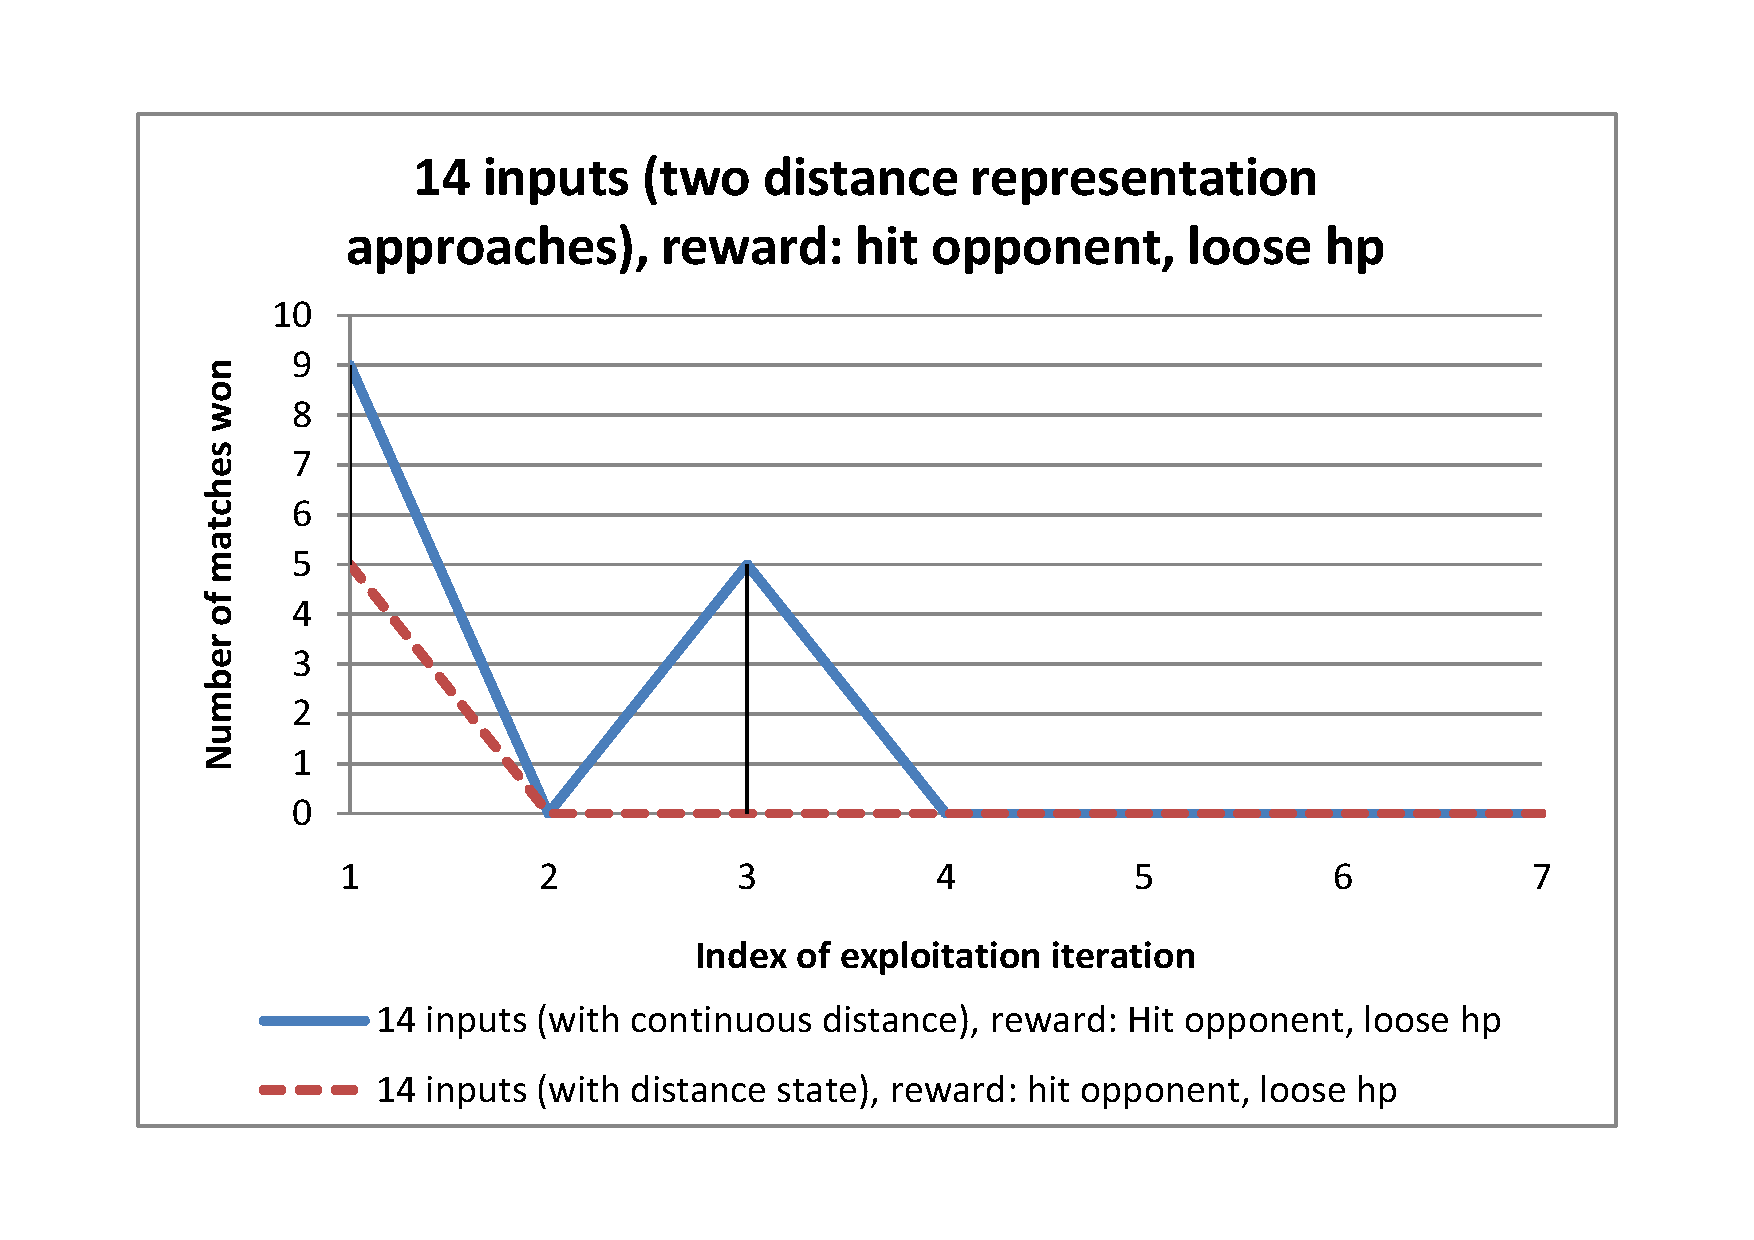
\includegraphics[width=1.0\columnwidth]{fig_ql_14_r1}}
\caption{Results of tests: 14 inputs (two distance representation approaches), reward: Hit opponent, loose hp}
\label{fig:first}
\end{figure}
%%
\\ \hphantom{x}
We decided to turn in the rewarding mechanism changes direction. Once more two previously tested representations were used but with \emph{Unit hp comparison} approach. Also a small change were made to representation - we decided to drop top speed input as well in order to smaller representation. This time one of the results appeared to be promising and is presented on Fig.\ref{fig:third}.
\begin{figure}[htp]
\centerline{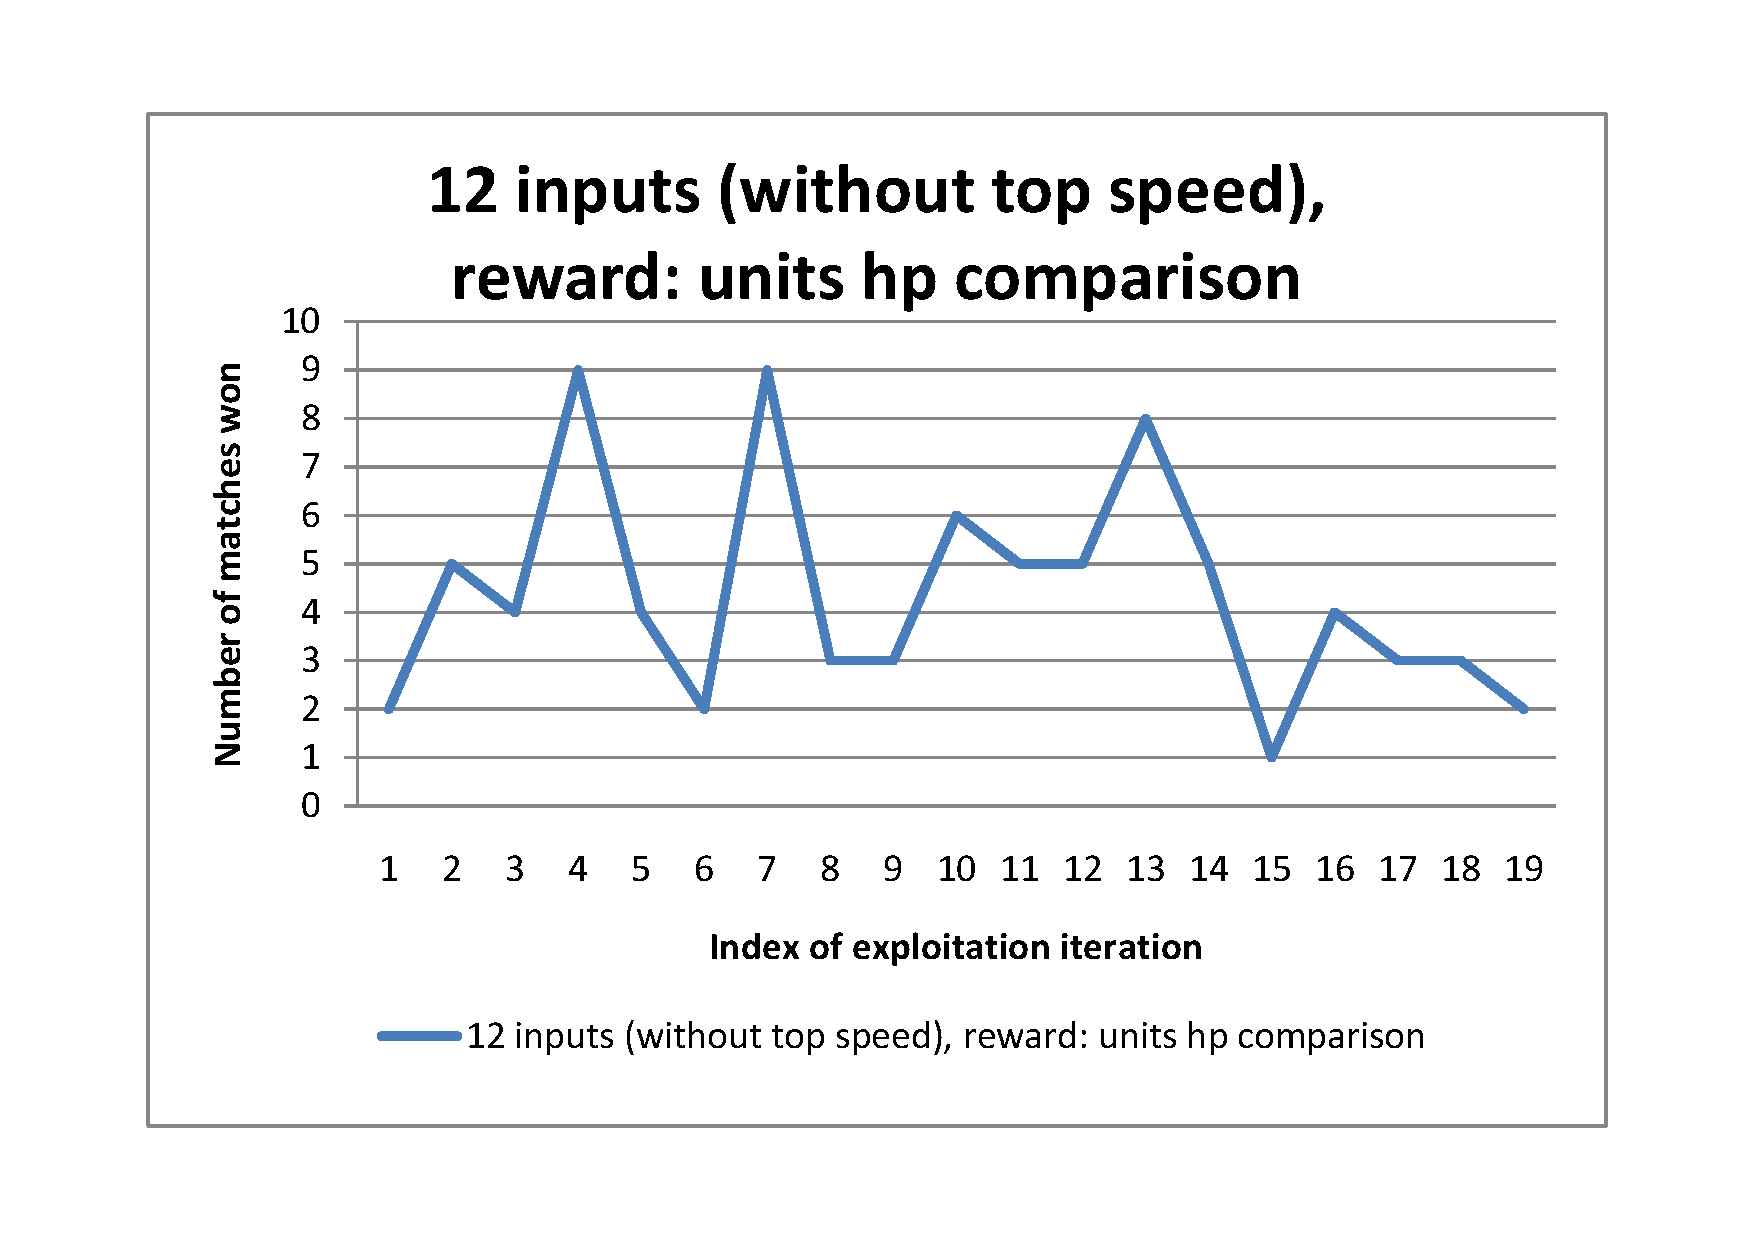
\includegraphics[width=1.0\columnwidth]{fig_ql_12(-ts)_r2}}
\caption{Results of test: 12 inputs (without top speed), reward: Hit opponent, loose hp}
\label{fig:third}
\end{figure}
%%
\\ \hphantom{x}
At this figure we can see that in first few iterations bot starts to learn some strategy - winning rate is rising, but later winning rate starts floating from 2 won matches up to 9 won matches. At the end winning rate starts to strive for zero. Once more selected state representation and reward mechanism appears to be not a good combination.
\\ \hphantom{x}
In order to receive more information, more excluding certain inputs and switching rewarding mechanism tests were provided. Unfortunately, the results were not satisfying, however enabled us to understand bot working mechanisms better.
\\ \hphantom{x}
At the end we decided to rearrange reward mechanism entirely and also smaller representation state. The final version included only 7 inputs: \emph{Previous action},\emph{ Health}, \emph{Current cooldown} and\emph{ Distance to enemy}. The rewarding mechanism, instead of approaches with small reward value, were changed into \emph{Modified comparison} mechanism. Both this changes allowed to achieve promising and effective results presented on Fig.\ref{fig:nnfr} and Fig.\ref{fig:nnff}. From those figures we are able to perceive learning process. More comment on results of this test is to be found in next section (NN structure experiments) under 7-3-1 neural network structure test.
\\
\subsubsection{QL parameters experiments}\hfill \\ \hphantom{x}
Q learning in our implementation requires two parameters: discount factor which is a multiplier factor for maximum future value and $\varepsilon$ which is a $\varepsilon$-greedy mechanism parameter. \\ \hphantom{x}
Tests with first mentioned parameter revealed that with it's increasing value teaching abilities of reinforcement learning increases. With the discount factor of value 0.5 neural network was not able to learn proper wining strategy - the only strategy the bot came up with was attacking for a short time and withdrawing a little. Theoretically this strategy might be a good one, but during the real match bot was not able to perform all this actions in a way so this strategy would be effective - bot was dying most of matches. We achieved best results with a discount factor of value 0.9. \\ \hphantom{x}
Testing $\varepsilon$ parameter revealed that with it's bigger value bot's performance weakens. According to random bot, described in previous chapters where we shown that random player approach is entirely inefficient, we can notice that with $\varepsilon$ value rising QLearning bot becomes more similar to random player and it's performance drops. Therefore we decided to set the $\varepsilon$ value to 0.01.
\\
\subsubsection{NN structure experiments}\hfill \\ \hphantom{x}
For the purpose of these tests four cases of neural network structure were provided:
\begin{itemize}
\item 7in-3-2-1out
\item 7in-7-1out
\item 7in-1-1out
\item 7in-3-1out
\end{itemize}
\hfill \\ \hphantom{x}
Testing methodology was iteration of 100 matches where first 80 were the exploration part and last 20 were the exploitation part. Based on data received this way we were able to create line graphs of won matches over all iterations played.
\\ \hphantom{x}
We decided to start our test with a structure of 7 inputs, 3 middle layer neurons and 1 output which in our opinion was most suitable structure for this issue. The results from test are presented on Fig.\ref{fig:nnfr}. From that figure we can see that at first approximately 16 iterations bot goes through the learning process. To make this process more visible, first 22 iterations are presented on Fig.\ref{fig:nnff}. Rest of the iterations results of exploitation part are floating around value of 11.
\hfill \\ \hphantom{x}
\begin{figure}[htp]
\centerline{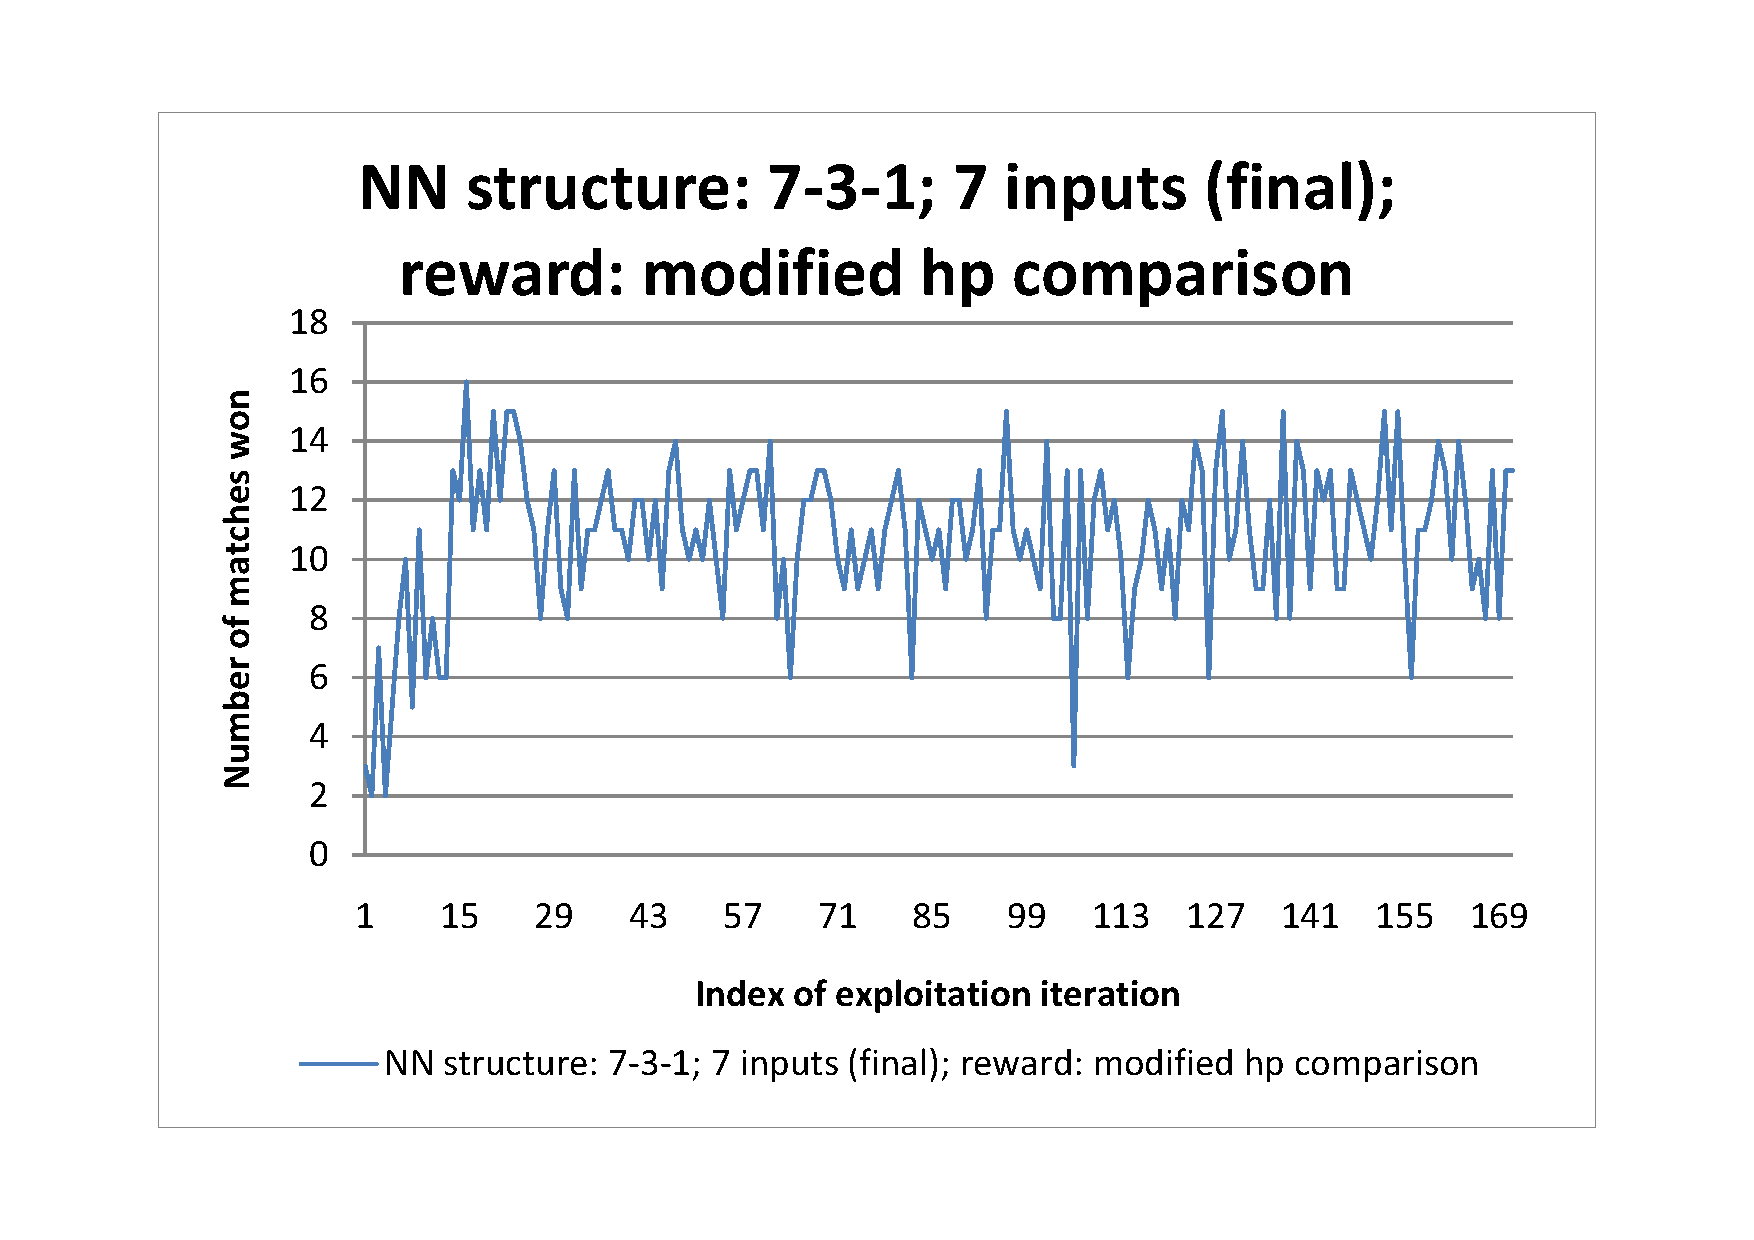
\includegraphics[width=1.0\columnwidth]{fig_ql_731_7(f)_r3_all}}
\caption{Results of test with neural network structure: 7in-3-1out}
\label{fig:nnfr}
\end{figure}
%%
\begin{figure}[htp]
\centerline{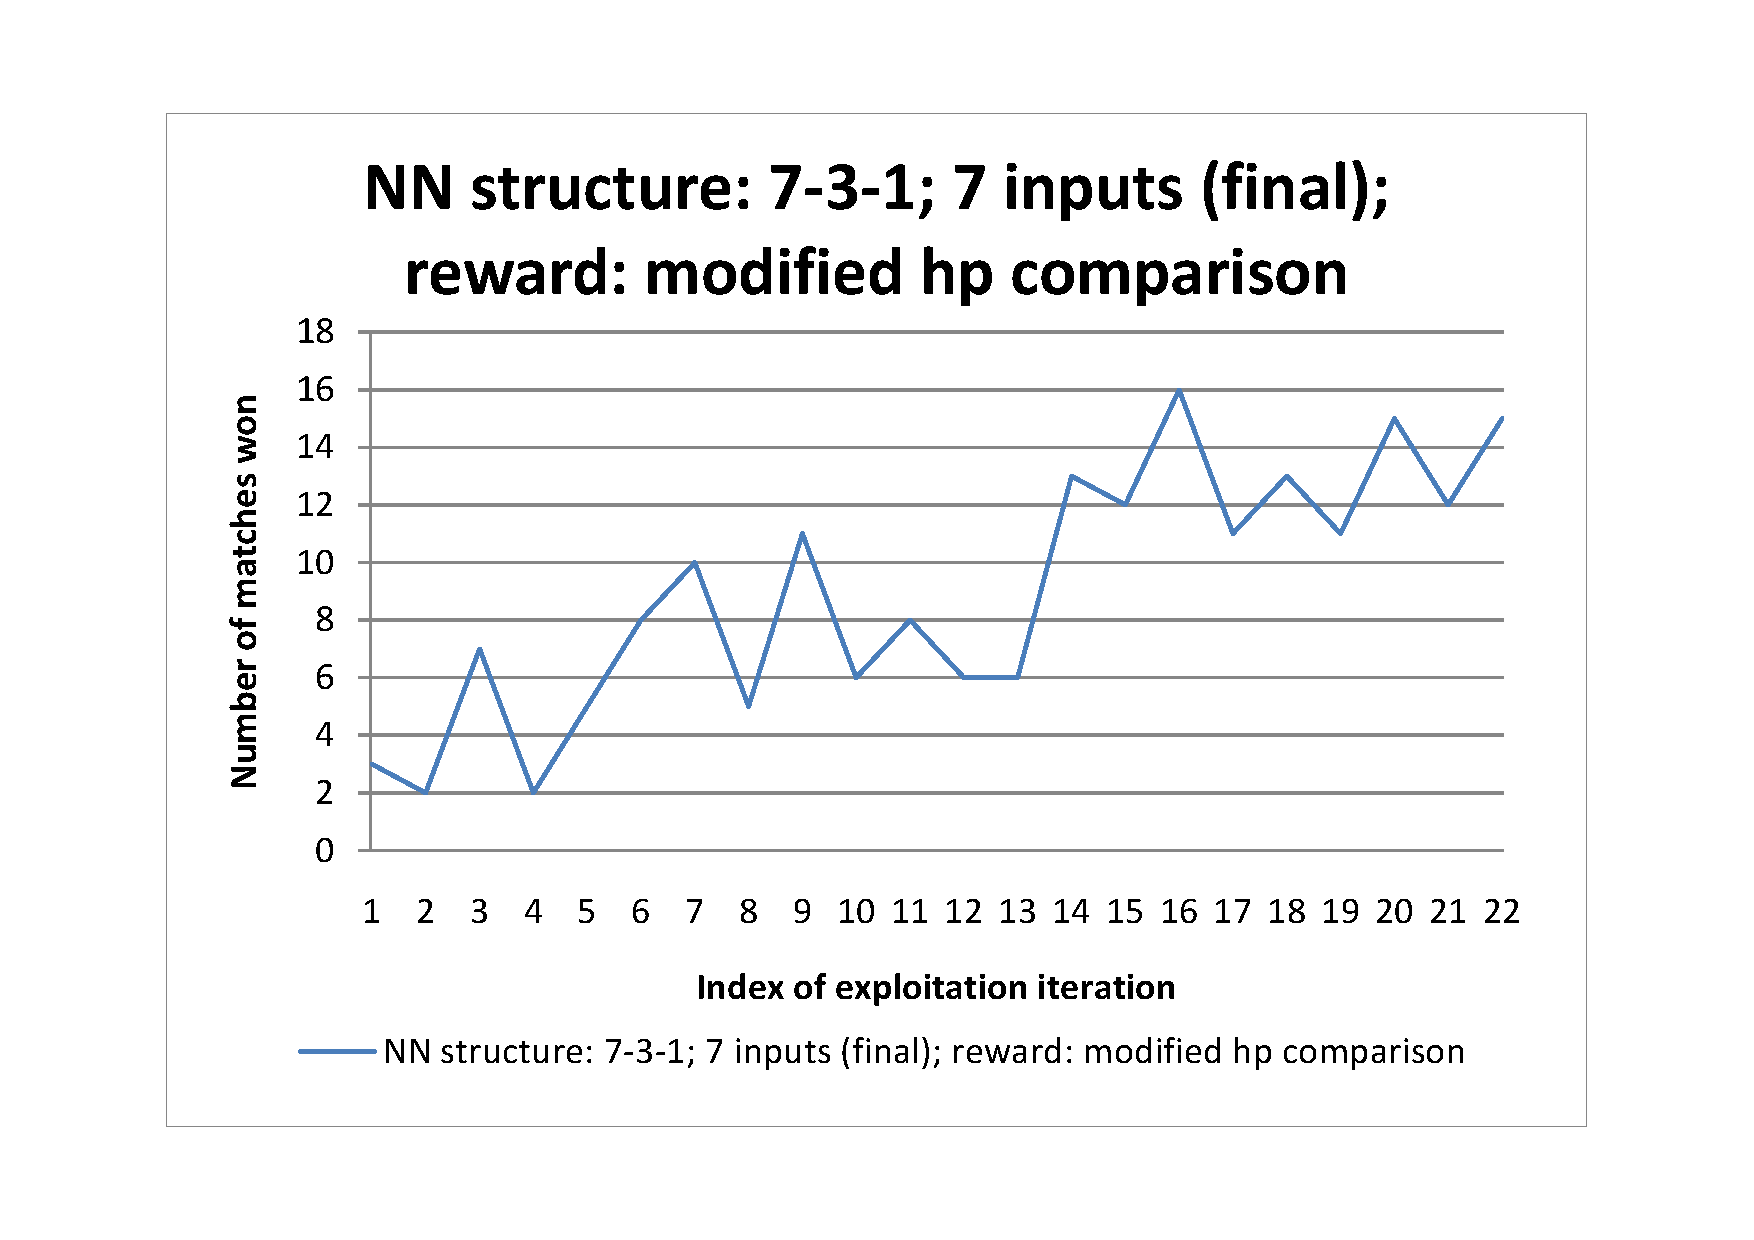
\includegraphics[width=1.0\columnwidth]{fig_ql_731_7(f)_r3_first20}}
\caption{First 22 iterations of results of test with neural network structure: 7in-3-1out}
\label{fig:nnff}
\end{figure}
%%
\hfill \\ \hphantom{x}
The strategy that bot learned was basically to move forward until enemy step inside bot unit weapon range and not to move during fire exchange. From algorithm point of view, bot learned that the best strategy is to give attack order.
\\ \hphantom{x}
Next tests were provided also for only one hidden layer, but with a different number of neurons in it in order to check it's impact on bot performance.
\\ \hphantom{x}
First of one hidden layer tests was test  with a neural network structure of 7 inputs, 7 neurons hidden layer and one output. The results of this test are presented on Fig.\ref{fig:nnt}. We can see that the results are a little unexpected. There is no visible learning process - at the beginning exploitation results are between 1 and 16 won matches, although with time they are tending to value of 9.
\begin{figure}[htp]
\centerline{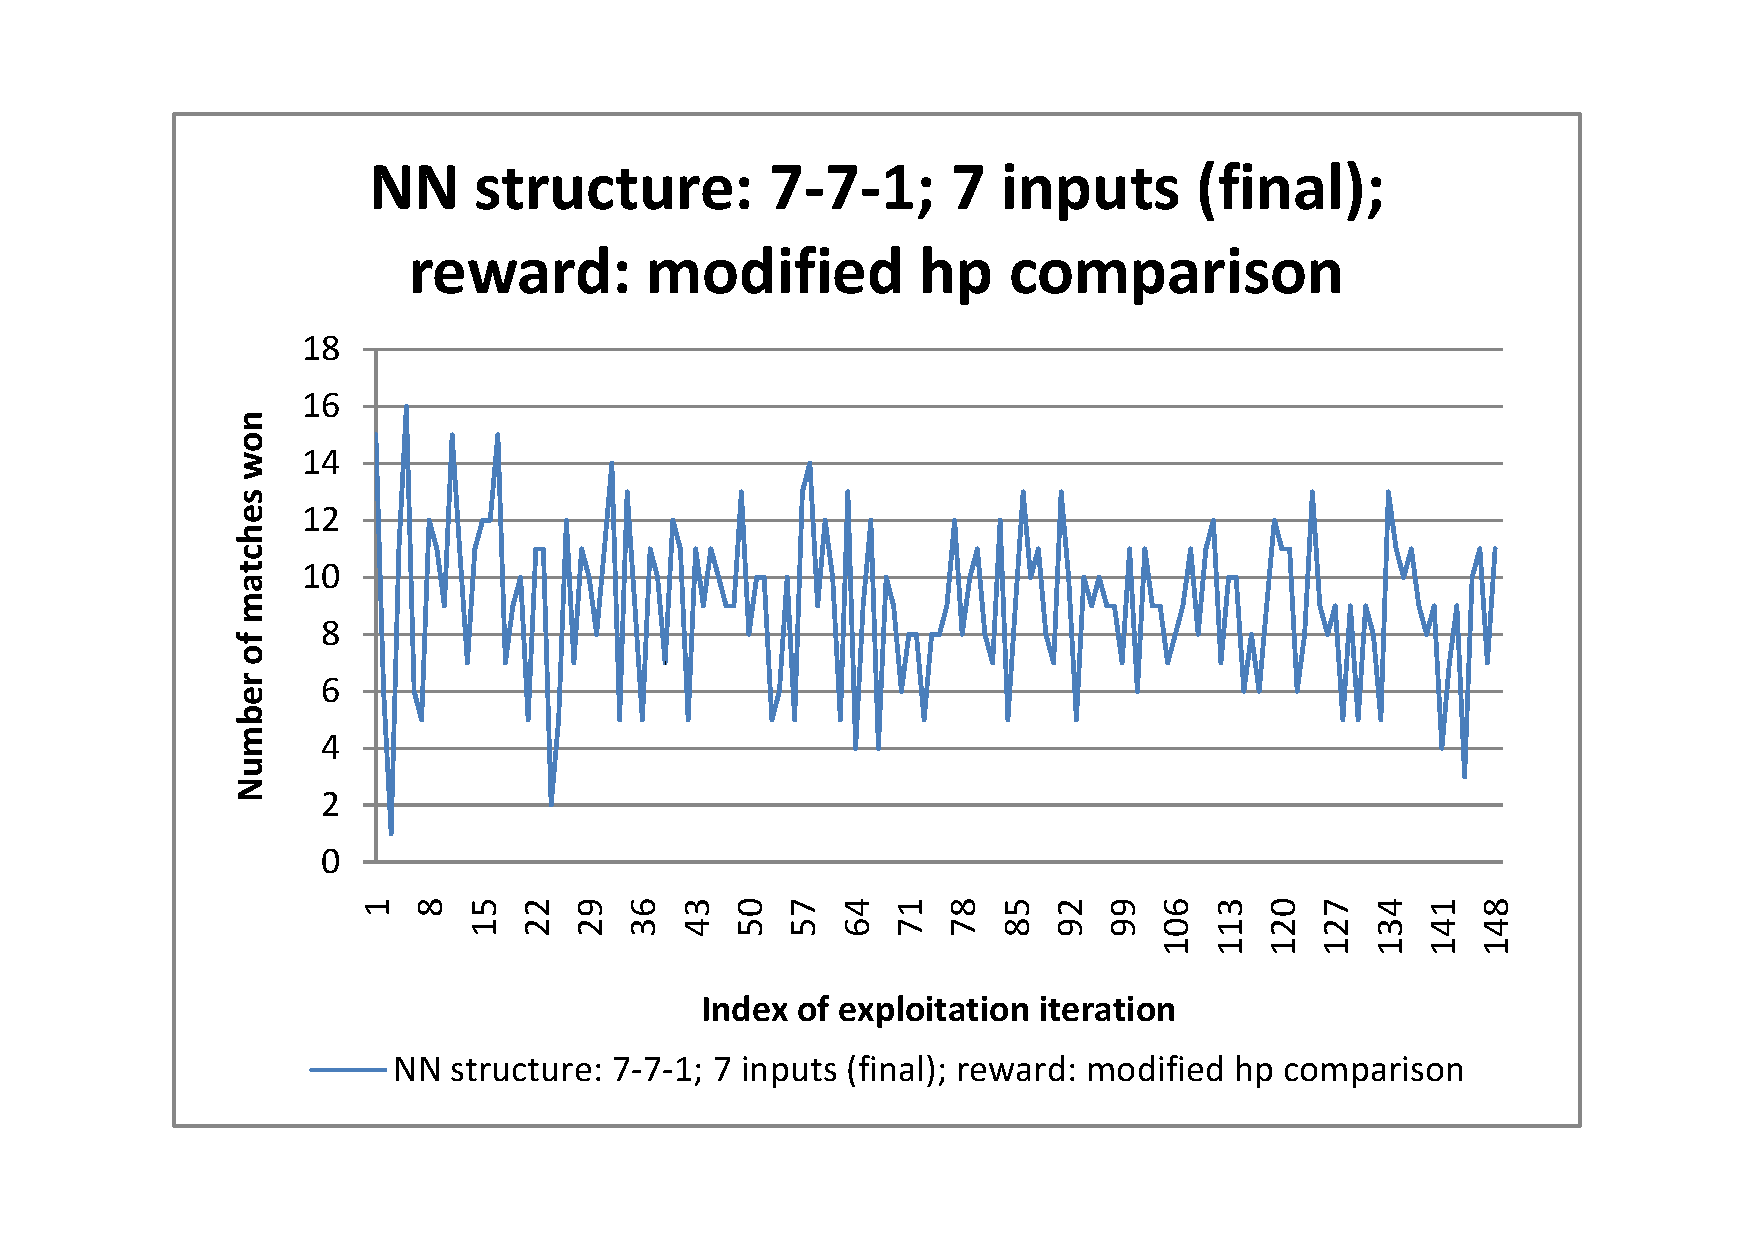
\includegraphics[width=1.0\columnwidth]{fig_ql_771_7(f)_r3}}
\caption{Results of test with neural network structure: 7in-7-1out}
\label{fig:nnt}
\end{figure}
%%
\hfill \\ \hphantom{x}
Again, bot came up with strategy to move forward and attack enemy as soon as he will step inside it's unit weapon range and not to move during fire exchange which is again a strategy to give attack order all the time.
\\ \hphantom{x}
Next test brought also a little unexpected results. The neural network with structure of 7 inputs, 1 neuron in middle layer and one output appeared also tend to value of 9 matches won in one iteration and also no learning process is visible. However in case of this neural network structure, learning process is very fast due to very simple structure - neural network contains only two neurons. \\ \hphantom{x}
The second surprising fact was that a bot with that small amount of neurons is able to get to learn a strategy that allows him to win matches. Basically the bot learned to wait for enemy to enter it's weapon range and than start to shoot and not to move during fire exchange. The interesting difference from previous bots is also the fact that this bot achieves this waiting strategy in different ways: one time he just wait at it's starting position for enemy bot, but other times he withdraws for some time and then wait for enemy.
\begin{figure}[htp]
\centerline{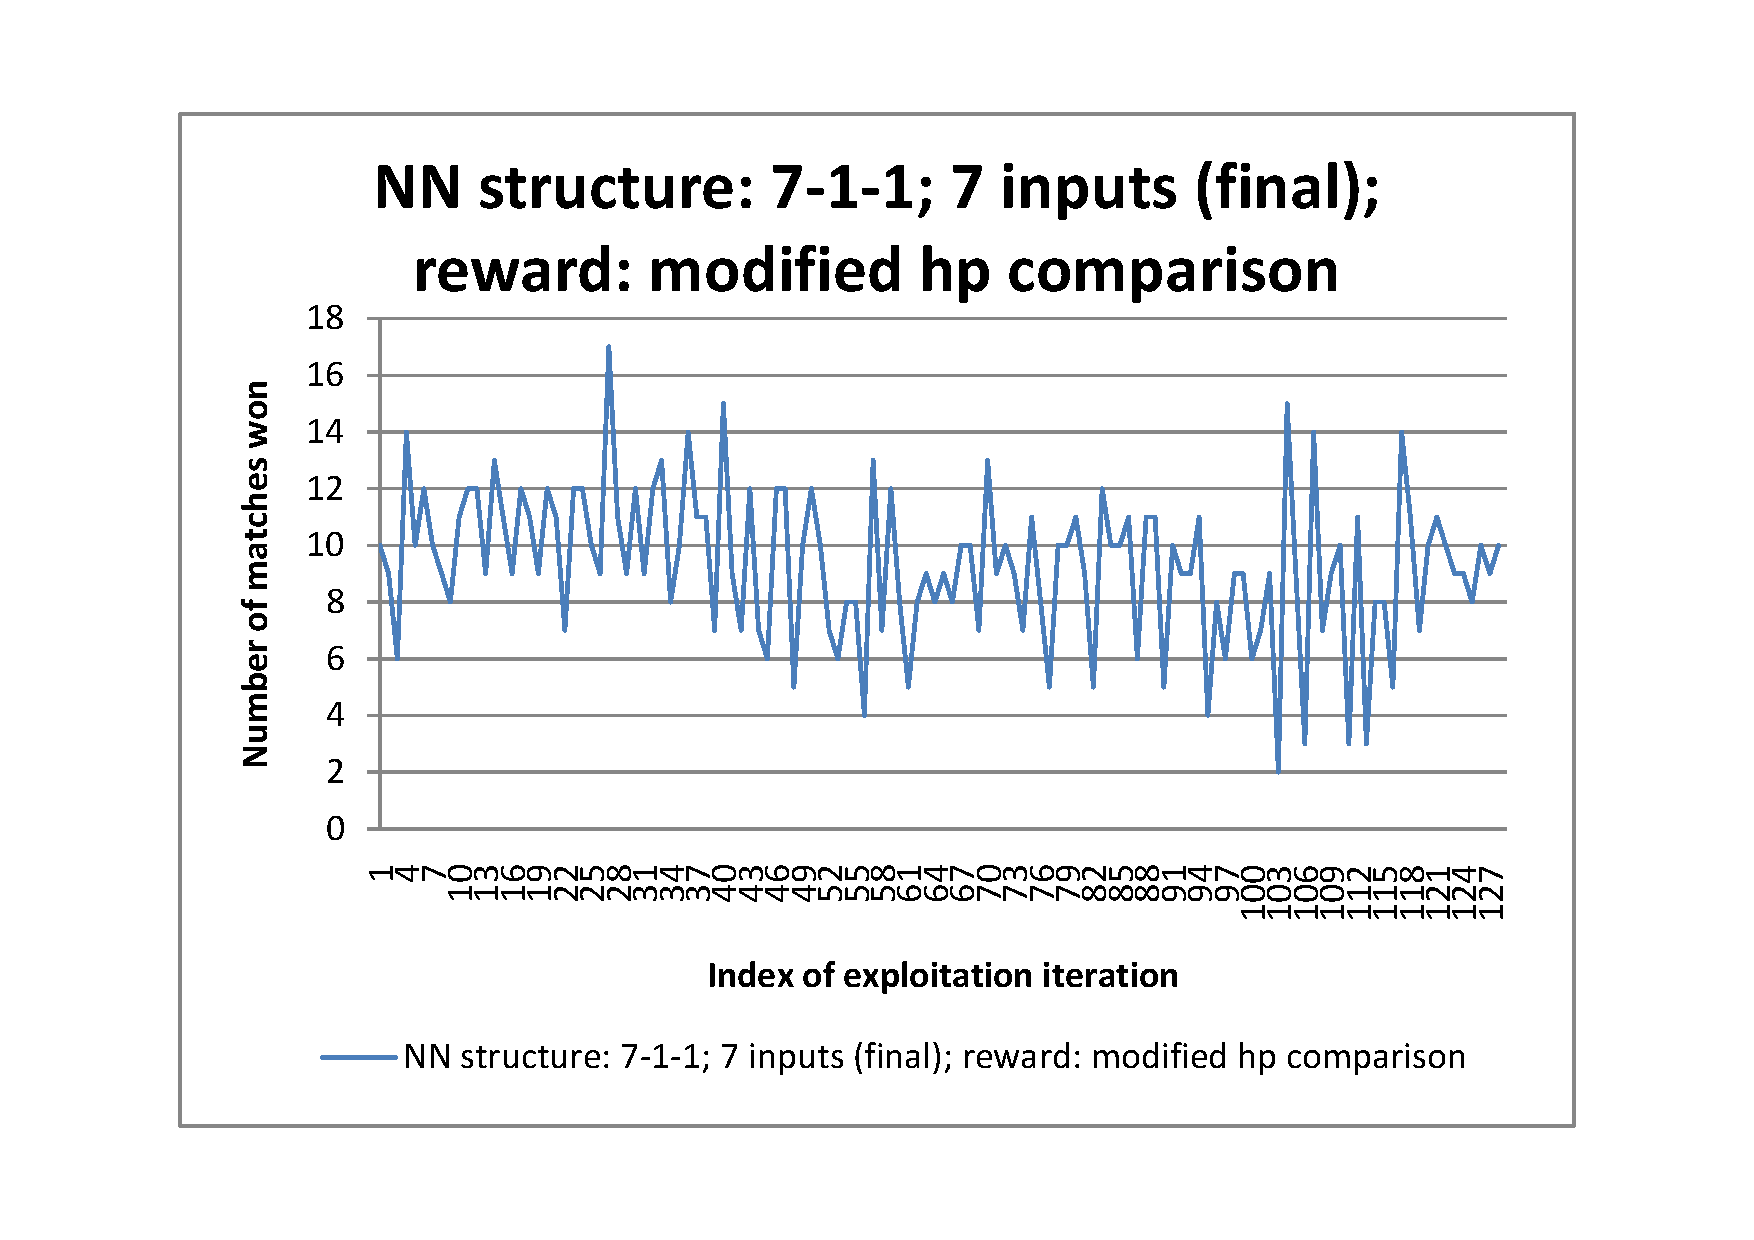
\includegraphics[width=1.0\columnwidth]{fig_ql_711_7(f)_r3}}
\caption{Results of test with neural network structure: 7in-1-1out}
\label{fig:nns}
\end{figure}
%%
\\ \hphantom{x}
At the end we also wanted to test bot with neural network of two hidden layer structure of 7 inputs, 3 neurons in first hidden layer, 2 neurons in second hidden layer and 1 output. The purpose of this test was to prove that adding more middle layers would not improve bot performance. The results are shown on Fig.\ref{fig:nnf} and allows us to see that bot starts to learn in approximately first 8 iterations and than it starts floating in range between 5 to 16 won games in iteration.
\begin{figure}[htp]
\centerline{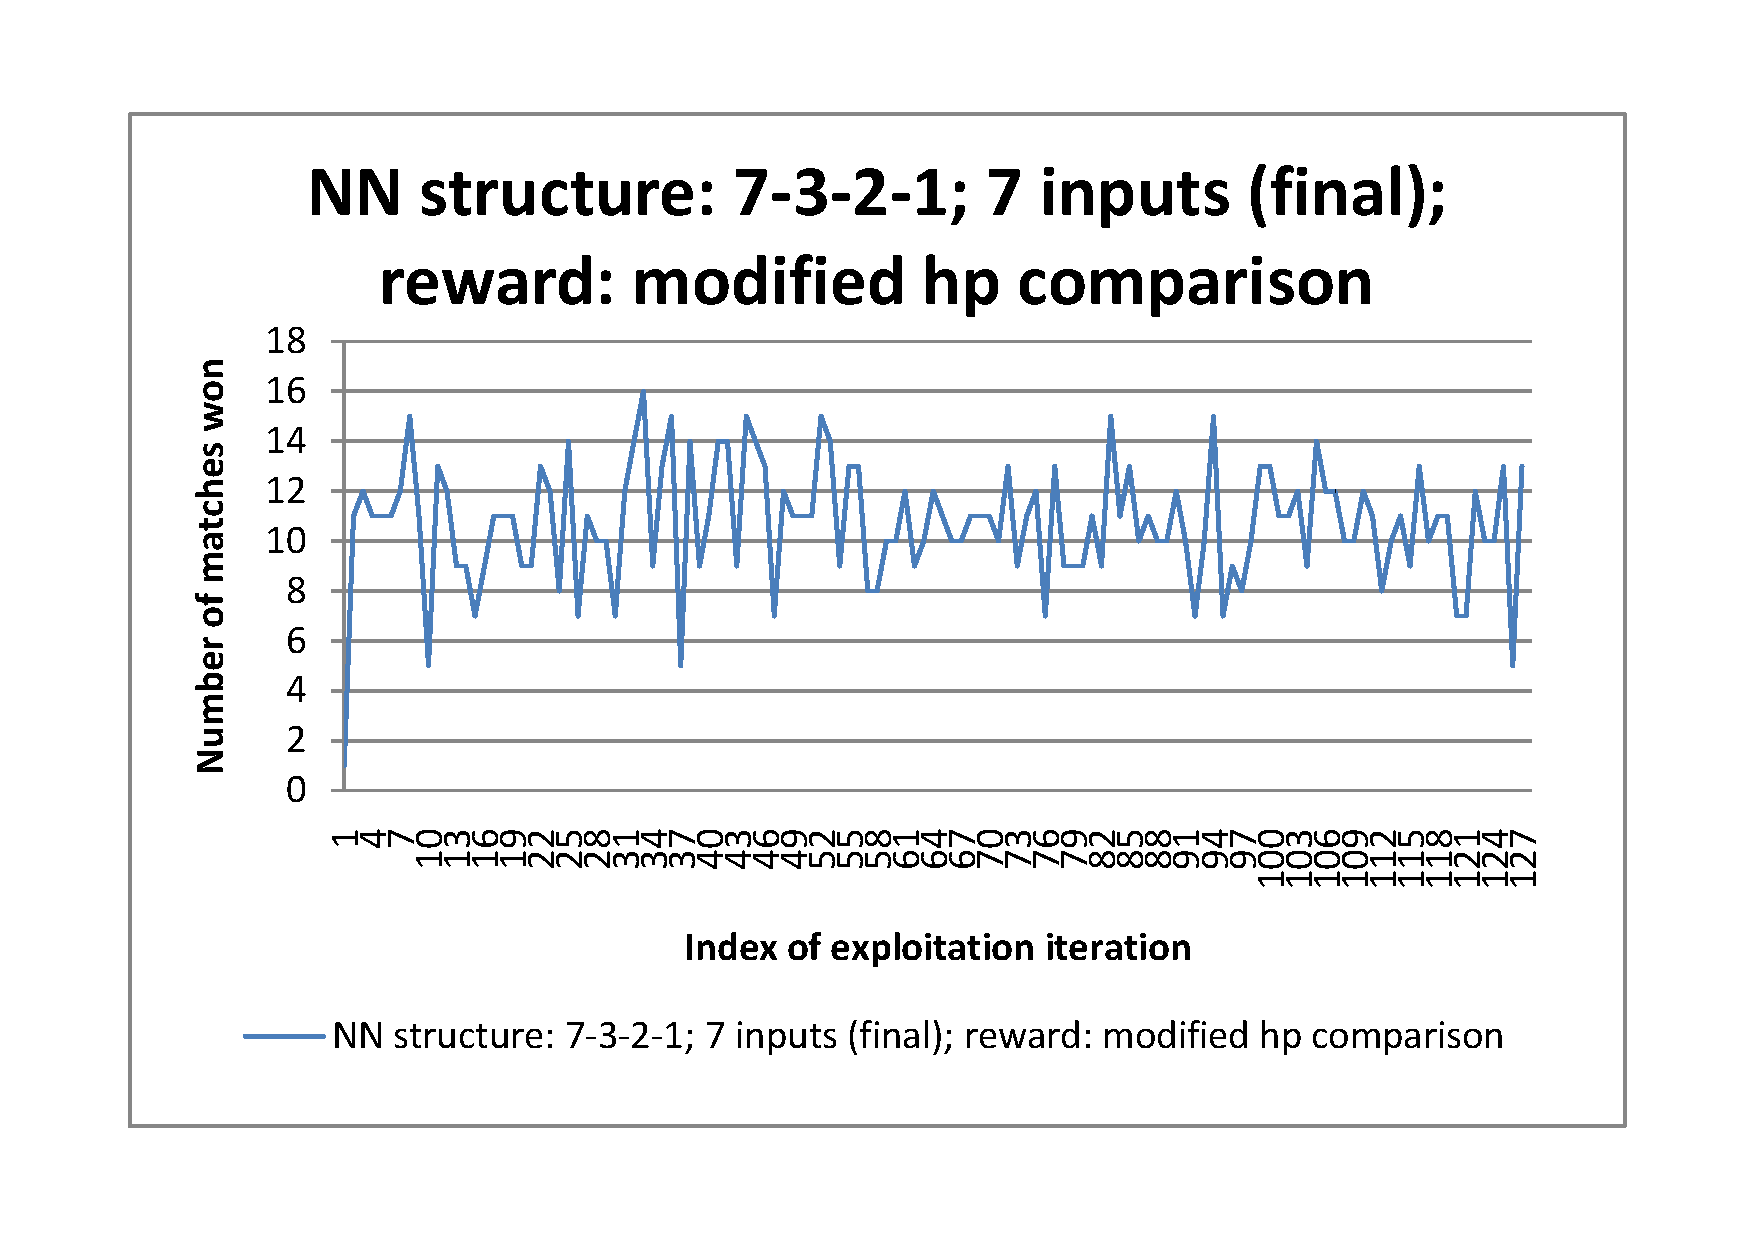
\includegraphics[width=1.0\columnwidth]{fig_ql_7321_7(f)_r3}}
\caption{Results of test with neural network structure: 7in-3-2-1out}
\label{fig:nnf}
\end{figure}
%%
\hfill \\ \hphantom{x}
The behavior of this last bot tested was similar to first two tested (bots 7-3-1 and 7-7-1).
\\ \\ \hphantom{x}
To summarize section about NN structure experiments, we would also like to discuss a floating aspect of all tests in this section. We discovered that game contain independent (in meaning that we do not have possibility to affect it) factor which affects match result.
\\ \hphantom{x}
This factor is an issue of who starts to shoot first. The problem is, that due to fact that both fighting units are of the same type, the unit who start to shoot first will definitely win the match. Theoretically there is 50\% chance for each unit to perform this operation first so this factor has a huge impact on match result.
\\ \hphantom{x}
From performed tests we can see that this factor is affecting about half of the games - all obtained results showed on line graphs indicates that the number of matches won in each iteration is floating around value of 10 which is half of all exploitation matches played in iteration.
%%%

%-------------------------------------------------------------------------------------------------------------------------------------------------
\subsection{T-tests} \hfill \\ \hphantom{x}
T-test were made in comparison to bot with structure of 7-3-1 for all other different neural network structure bots that were tested. We used two-tailed tests. Tests are based on amount of hit points left on board - at the end of a match bot unit hit points and enemy unit hit points are subtracted and normalized by greater of maximum fighting units hp value as it is shown at following formula:
\begin{IEEEeqnarray}{rCl}
hp\_left = \frac{uhp-ehp}{\max\{muhp,mehp\}},
\label{equation:reward}
\end{IEEEeqnarray} 
where:\\
uhp - unit hit points,\\
ehp - enemy unit hit points,\\
muhp - maximum unit hit points,\\
mehp - maximum enemy unit hit points.\\ \hphantom{x}
This formula provides output values in range from -1 to 1, where -1 is 100\% enemy unit hit points and 1 is 100\% bot unit hit points.
%
\\ \hphantom{x}
T-test results are shown in table \ref{table:ql_ttest}. Row $\mu$ is a sample mean value, row $\sigma$ is a sample standard deviation value, p-value can be found in $p$ row. The \emph{hypothesized mean} is a mean value for bot with 7-3-1 neural network structure (marked with a \emph{(ref)}) .
% ---------
\begin{table}
\caption{T-test values table}
\begin{center}
\begin{tabular}{|l|r|r|r|r|}
\hline
\multicolumn{1}{|c|}{\bf T-test } & 
\multicolumn{1}{|c|}{\bf 7-3-1 (ref) } & 
\multicolumn{1}{|c|}{\bf 7-1-1 } & 
\multicolumn{1}{|c|}{\bf 7-7-1 } & 
\multicolumn{1}{|c|}{\bf 7-3-2-1 } \\
\hline
{\it $\mu$} &          0.007501 &        -0.006933 &          -0,094653 &       0.004547 \\
\hline
{\it $\sigma$} &          0,112205 &      0,110452 &          0,224809 &          0.127824 \\
\hline
{\it $p-value$} &          - &       1.02 $\times$ 10$^{-10}$ &          8.106 $\times$ 10$^{-123}$ &          0.2442 \\
\hline
\end{tabular}  
\label{table:ql_ttest}
\end{center}
\end{table}
% ---------
%%%

%-------------------------------------------------------------------------------------------------------------------------------------------------
\subsection{Discussion} \hfill \\ \hphantom{x}
The results of different neural network structure bots compared in table \ref{table:ql_ttest} with a t-test allows us to see structure impact to bot's performance. Bots with structures of 7-7-1 and 7-1-1 appeared to be significantly worse than referenced bot. The null hypothesis is rejected with significance level of 1\%. Contrary to expectations, a two hidden layer bot appeared to be second best with the null hypothesis not rejected even with a significance value of 10\%. Based on mean values of \emph{hit points left on board}, the best neural network structure appeared to be first tested (7-3-1), but wen we take into account learning speed, unexpectedly a bot with two hidden layers is better with approximately 8 learning iterations while 7-3-1 bot needed approximately 16. \\ \hphantom{x}
%
During tests it occurred that the best tactic in order to win a match is to provide only attack decisions at least during the fire exchange. \\ \hphantom{x}
%
The biggest problems we found were during the first preliminary tests with both state representation and reward mechanism. It took us a long time to find final solution. First attempts of small value rewards during the match were unsuccessful - values were to small and also targets of rewards inaccurate. In state representation the most problematic input occurred to be distance between fighting units. We tried three different approaches before we found the right one. \\ \hphantom{x}
%
As for further improvements, our bot could be expanded in a way that would enable to provide fights between different kinds of units of all races. This expansion would require to include additional inputs connected with other than Terran units statistics as shield of Protoss units for example. However, the balance of Starcraft game is so well designed that most of one versus one unit fights are from top doomed to end in a certain way. For example zergling unit will always loose against marine unit and marine unit will always loose against zelot unit. Therefore the only purpose of modifying implemented QLeqrning bot would be for symmetrical fights. \\ \hphantom{x}
%%%